%--------------------------------------
% Master's Thesis Title Page 
% LaTeX Template
% Version 1.0 (23/05/14)
%---------------------------------------

%----------------------------------------------------------------------------------------
%	PACKAGES AND OTHER DOCUMENT CONFIGURATIONS
%----------------------------------------------------------------------------------------

\documentclass[a4paper]{report}
\usepackage{helvet}
\usepackage{subfig}
\usepackage[toc,acronym,nomain]{glossaries} 
\usepackage{graphicx} % Displaying pictures in the document.
\usepackage[floatrow]{chemstyle} % Displaying figures next to item lists.
\usepackage[hidelinks]{hyperref}
\usepackage{listings} % Adding source code listings.
\usepackage{color}
\usepackage{gensymb}
\usepackage{mathtools}

\newglossaryentry{js} 		{ name=JavaScript,	description={A scripting language used in web development}}
\newglossaryentry{cpp} 		{name=C++, description={A object-oriented programming language.}}
\newglossaryentry{sc} 		{name=SystemC, description={A simulation library building on C++}}
\newglossaryentry{sampa}  {name=SAMPA, description={SAMPA ASIC}, plural=SAMPAs}
\newglossaryentry{vhdl}{name=VHDL,  description={A Hardware description language}}
\newglossaryentry{verilog}{name=Verilog, description={A Hardware description language}}
\newglossaryentry{altro}{name=ALTRO, description={ALTRO ASIC}}
\newglossaryentry{zs}{name=Zero Suppression, description={Suppression schema/algorithm}}
\newglossaryentry{pq}{name= Priority Queue, description={Datastructure which sorts elements based on a priority(numerical value)}}
\newglossaryentry{rng}{name= Random Number Generator, description={Computational device designed to generate numbers that lack a pattern}}

\newacronym{lhc}{LHC}{Large Hadron Collider}
\newacronym{cern}{CERN}{European Organization for Nuclear Research}
\newacronym{alice}{ALICE}{A Large Ion Collider Experiment}
\newacronym{tpc}{TPC}{Time Projection Chamber}
\newacronym{tev}{TeV}{Tera Electron Volt}
\newacronym{qcd}{QCD}{Quantum Chromodynamics}
\newacronym{asic}{ASIC}{Application Specific Integrated Circuits}
\newacronym{rcu}{RCU}{Readout Control Unit}
\newacronym{cru}{CRU}{Common Readout Unit}
\newacronym{gbt}{GBTx}{Giga Bit Transceiver}
\newacronym{fec}{FEC}{Front-End Card}
\newacronym{fifo}{FIFO}{First-In-First-Out}
\newacronym{gem}{GEM}{Gas Electron Multiplier}
\newacronym{mwpc}{MWPC}{Multi Wire Proportional Chamber}
\newacronym{fpga}{FPGA}{Field-Programmable Gate Array}
\newacronym{bt}{BT}{Binary Tree}
\newacronym{oop}{OOP}{Object-Oriented Programming}

\makeglossaries
\definecolor{mygreen}{rgb}{0,0.6,0}
\definecolor{mygray}{rgb}{0.5,0.5,0.5}
\definecolor{mymauve}{rgb}{0.58,0,0.82}

\lstset{ %
  backgroundcolor=\color{white},   % choose the background color; you must add \usepackage{color} or \usepackage{xcolor}
  basicstyle=\footnotesize,        % the size of the fonts that are used for the code
  breakatwhitespace=false,         % sets if automatic breaks should only happen at whitespace
  breaklines=true,                 % sets automatic line breaking
  captionpos=b,                    % sets the caption-position to bottom
  commentstyle=\color{mygreen},    % comment style
  deletekeywords={...},            % if you want to delete keywords from the given language
  escapeinside={\%*}{*)},          % if you want to add LaTeX within your code
  extendedchars=true,              % lets you use non-ASCII characters; for 8-bits encodings only, does not work with UTF-8
  frame=single,                    % adds a frame around the code
  keepspaces=true,                 % keeps spaces in text, useful for keeping indentation of code (possibly needs columns=flexible)
  keywordstyle=\color{blue},       % keyword style
  language=Octave,                 % the language of the code
  morekeywords={public, if, for, else, class, import, return, null},            % if you want to add more keywords to the set
  numbers=left,                    % where to put the line-numbers; possible values are (none, left, right)
  numbersep=5pt,                   % how far the line-numbers are from the code
  numberstyle=\tiny\color{mygray}, % the style that is used for the line-numbers
  rulecolor=\color{black},         % if not set, the frame-color may be changed on line-breaks within not-black text (e.g. comments (green here))
  showspaces=false,                % show spaces everywhere adding particular underscores; it overrides 'showstringspaces'
  showstringspaces=false,          % underline spaces within strings only
  showtabs=false,                  % show tabs within strings adding particular underscores
  stepnumber=1,                    % the step between two line-numbers. If it's 1, each line will be numbered
  stringstyle=\color{mymauve},     % string literal style
  tabsize=2,                       % sets default tabsize to 2 spaces
  title=\lstname                   % show the filename of files included with \lstinputlisting; also try caption instead of title
}
%----------------------------------------------------------------------------------------
%	TITLE PAGE
%----------------------------------------------------------------------------------------

\newcommand*{\titlePage}{\begingroup % Create the command for including the title page in the document
\fontfamily{phv}\selectfont
\centering % Center all text

\vspace{200pt}
{\Huge Lorem ipsum dolor sit amet} \\ % Title
\vspace{5pt}

{\Large \textsl{Consectetur adipisicing elit, sed do tempor incididunt ut labore et dolore magna aliqua}} % Subtitle or further description
\vspace{50pt}

{\Large{H\r{a}vard Rustad Olsen}}\\ % Author name

\vfill % Whitespace between the author name and the publisher logo

{\Large Master's thesis in Software Engineering at \\
\vspace{10pt}
Department of Computing, Mathematics and Physics, \\
Bergen University College \\
\vspace{10pt}
Department of  Informatics, \\
University of Bergen \\}
\vspace{10pt}
{\large June 2015} % Month and year published

\begin{figure}[h!]
	\captionsetup[subfigure]{labelformat=empty}
	\subfloat[][]{
\includegraphics[width=50pt]{HIB_sort_hovedlogo.eps}}
	\hfill
	\subfloat[][]{
\includegraphics[width=50pt]{uib-logo.eps}}
\end{figure}


\endgroup}

%----------------------------------------------------------------------------------------
%	BLANK DOCUMENT
%----------------------------------------------------------------------------------------

\begin{document} 

\pagestyle{empty} % Removes page numbers

\titlePage % This command includes the title page

\newpage

\chapter*{Acknowledgements}
\addcontentsline{toc}{chapter}{Acknowledgments}

\paragraph{•}
Håvard Helstrup, Johan Alme, Dieter, Arild, Christian, (Damian).
\newpage

\phantomsection
\addcontentsline{toc}{chapter}{Contents}
\tableofcontents

\newpage
\phantomsection
\addcontentsline{toc}{chapter}{List of Figures}
\listoffigures

\newpage
\phantomsection
\addcontentsline{toc}{chapter}{List of Tables}
\listoftables

\newpage
\chapter*{List of Algorithms}
\addcontentsline{toc}{chapter}{List of Algorithms}

\newpage
\chapter*{Listings}
\addcontentsline{toc}{chapter}{Listings}
\newpage

% Glossary
%\chapter*{Glossary and acronyms}
%\addcontentsline{toc}{chapter}{Glossary and acronyms}
\printglossaries
\newpage

\chapter{Introduction}
\textit{This chapter will cover the motivation, as well as the scope and goal of this report.}

\section{Motivation}
\label{sec:motivation}
\paragraph{•}
The \gls{lhc} at the \gls{cern} is the world's largest particle accelerator, hosting multiple ongoing experiments.
After a run period of more than 3 years, the \gls{lhc} at the \gls{cern} will be shut down for about 18 months.\cite{ls2}
The purpose of this shutdown is to do maintenance on various equipment in the \gls{lhc}, as well as significant upgrades to the different detectors, one of which is the detector for the \gls{alice} experiment.
\gls{alice} consists of multiple sub-detectors, which combined collects an enormous amount of data.
This amount is expected to increase after the shutdown period as the interaction rate of the \gls{lhc} will increase.
Due to the increase in data output, the \gls{alice} collaboration is seeking to upgrade and enhance the detectors capabilities.\cite{alice-upgrade}
This includes a partial redesign of the readout electronics, upgrades to multiple sub-detectors and additional hardware upgrades.

\paragraph{•}
The \gls{alice} detectors main device for tracking and identifying particles is the \gls{tpc} sub-detector.
A starting/temporary? design for the new \gls{tpc} readout electronics is made, and the different components are currently being developed.
As this is still being worked on, many questions about the different components are yet to be answered.
Are the current specifications sufficient to handle the expected increase in output from the detector?
Do they have the necessary bandwidth to be able to send the data with minimal sample loss.
Are the buffer memory enough to handle the traffic.
Is it possible to optimize the current solution in any way?

\paragraph{•}
The previous paragraph motivates us to find a reliable way of determining a sufficient design for the readout electronics, while being both time and cost efficient.
One strategy for solving this problem, which will be further explored in this thesis is creating a simulation of the system.
Doing a simulation requires designing a accurate representation of the readout electronics, and creating a testbench where it is possible to configure and run multiple tests.


\section{Research Question}

\paragraph{•}
Given the motivation and introduction given in section \ref{sec:motivation} the research question for this thesis becomes:

\paragraph{•}
Is it possible to design and implement a simulation which directly represent the readout electronics, and in doing so will it have an optimizing effect?

\section{Thesis goal}


\section{Report structure}
Chapter 2 will give the reader the background information to be able to understand the different academic and scientific terms used, as well as some information about the context of the report. This includes information about \gls{cern}, the \gls{alice} experiment and the physics most relevant to the thesis.
Chapter 3 is going further into the problem discussed in this report, initial plans on solving the problem, and information about the tools used.
Chapter 4 will talk about the implementation of the simulation, what problems occurred along the way, and the chosen solution. The chapter will go into the design, as well as code snippets from the implementation.
With the information given in chapter 4, chapter 5 will discuss the results of the different simulations run, and evaluate the solution.
Chapter 6 will conclude the thesis with some closing words, and work that can be done in the future.


\chapter{Background}
\textit{This chapter will give the reader the background needed to set the rest of the thesis in context.}

\section{CERN}
\paragraph{•}
\gls{cern} is a European research and scientific organization based out of Geneva near the Franco-Swiss border.\cite{cern}
\gls{cern} is a collaboration between 21 countries with a member staff of over 2500, and more than 12000 associates and apprentices.
The organization was founded in 1954 and has since than been the birthplace of many major scientific discoveries.
These are not limited to discoveries in the field of physics, but includes the creation of the World Wide Web.\cite{www}
Currently the biggest project at \gls{cern} is the particle accelerator, which serves as the foundation for multiple experiments in the field of particle physics.
% 2 - 3 more sentences about this!

\section{The Large Hadron Collider}
\label{sec:lhc}
\paragraph{•}
Starting up on 10 September 2008, \gls{lhc} is the latest construct added to \gls{cern}'s particle accelerator complex.\cite{lhc}
It consist of a 27 kilometre underground ring of superconducting magnets and accelerators which boost the energy of the particles travelling inside the collider.
The collider contains two adjacent parallel high-energy particle beams.
These beams consists of protons extracted from standard hydrogen atoms by stripping them of electrons.
Along the collider ring there are four intersect points where collision occurs.
Each point corresponds to the location of a particle detector - ATLAS, \gls{alice}, CMS and LHCb. 
The particle detectors are each built and operated by a large collaborations, with thousands of scientists from different institutes around the world.
The beams travel at close to the speed of light and are guided by a magnetic field, which is created and maintained by superconducting electromagnets.
Superconducting meaning that its in a state where it can most efficiently conduct electricity, without resistance or energy loss.
Achieving this state requires cooling the magnets to -271.3\degree~C , which is done by the distribution of liquid helium. 
The layout of the \gls{lhc} ring as well as its four collision points can be seen in \ref{fig:lhc}.

\begin{figure}[h!]
  \centering
    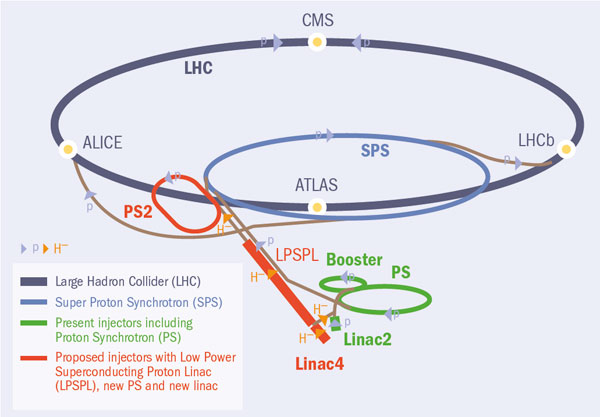
\includegraphics[width=0.7\textwidth]{images/lhc-ring.jpg}
     \caption{The Large Hadron Collider}
    \label{fig:lhc}
\end{figure}

\paragraph{•}
The beams travelling inside the \gls{lhc} reach an energy-peak of 7 \gls{tev}, which means that on impact with each other the collision reach an energy of 14 \gls{tev}.\cite{lhc-pdf}
During a normal run of the collider there will be about 600 million particle collisions per second during a period of 10 hours.
This leads to a huge amount of data for each of the detectors to read out. 
\gls{alice} is the detector which produce the most data, with about 1.25 GB/s.

\section{ALICE}
\subsection{Introduction}

\paragraph{•}
\gls{alice} is a so called heavy-ion detector, which means it studies collisions between particles of high energy.\cite{alice-home}
When the experiment started lead to lead ions collision was used, but they have now switched to colliding lead with protons, both produce a extreme high amount of temperature and density, but the later being the most preferable.
The high temperature and density is necessary to produce a phase of matter called quark-gluon plasma.

\subsection{Quark-gluon plasma}
\paragraph{•}
Shortly after the big bang, the universe was filled with a extremely hot cluster of all kinds of different particles moving around at near light speed.\cite{alice-physics}
Most of these particles was what is called quarks, fundamental building blocks for matter, and gluons which ties quarks together in order to form protons and neutrons.
Normally quarks and gluons are very strictly tied together, but in the conditions of extreme temperature and density as in the time shortly after the big bang, that are much more lousily coupled and free to move around in what is called quark-gluon plasma.
The existence of quark-gluon plasma and its properties is one of the key issues in \gls{qcd}.
The \gls{alice} collaboration studies this, observing how it behaves.

\subsection{The detector setup}
\paragraph{•}
The detector weighs in at 10,000 ton, it is 26 m long, 16 m wide, and 16 m high.\cite{alice-about}
It consists of 18 sub-detectors, each with its own set of tasks regarding tracking particles and collecting data.
This large number of sub-detectors are needed in order to get the full picture of the complex system which is being studied(e.i different types of particles).
The detector is also embedded in a magnetic field, created by a large solenoid magnet, which makes particles formed in collision bend according to its charge, and behave differently relative to its momentum. High momentum equals near straight lines while low momentum makes the particles move in spiral-like tracks.
During lead to lead collisions the collision rate peaks at 8 kHz(Where Hz is defined as number of events per second).
This number is still a lot lower in practice because the \gls{alice} detector uses a triggered based readout, which only triggers on head-on(central) collisions. 
The maximum readout rate of the current \gls{alice} detector is 500 Hz, which is more than enough to track central collisions.
\ref{fig:alice} shows a cross section of the detector as it is today with the red solenoid magnet, and all sub-detectors labelled.

\begin{figure}[h!]
  \centering
    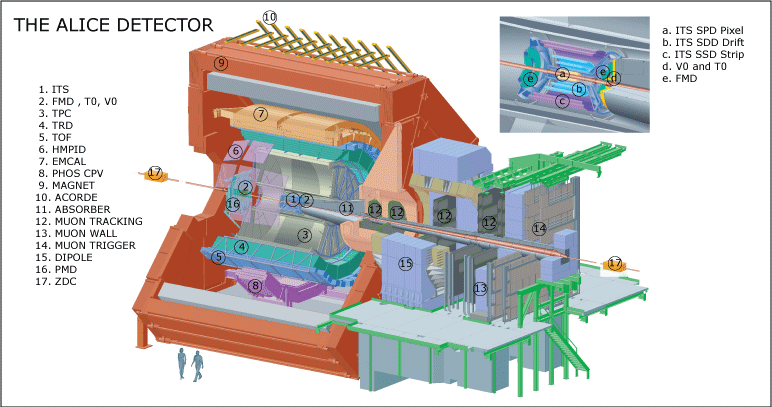
\includegraphics[width=1.0\textwidth]{images/alice-detector.png}
     \caption{The ALICE detector}
    \label{fig:alice}
\end{figure}

\section{The TPC detector}
\subsection{Intro}
\paragraph{•}
One of the most important sub-detectors, and the one that is relevant for this thesis is the \gls{tpc} detector. 
Located at the center of the \gls{alice} detector it is among the first entry point when gathering data from a particle collision.
It is a 88\(m^3\) cylinder filled with gas.
The gas works as a detection medium, which means that charges particles from a collision crossing will ionize the gas atoms, freeing electrons that move towards the end plates of the detector.
The readout is done by specially designed readout chambers, which is capable of handling the high amount of data produced in heavy-ion collisions.

\subsection{Readout electronics} %Should this be a chapter of itself?
\paragraph{•}
Signals from the readout chambers are passed along to the front-end readout electronics, which today consist of 4356 ALTRO chips.
The ALTRO chip is made up of 16 asynchronous channels that digitise, process and compress the analogue signals from the readout chambers.
It operates on a so called triggered readout mode.
In short when ALTRO receives the first trigger, it stores the following data stream into memory, holding on to it until it is ready to pass on the data. 
The front-end electronics are able to readout data at a speed of up to 300 MB/s.
\paragraph{•} %Legg til RCU i acronym
The ALTRO chip sends the digitised signals further down the readout chain to the readout control unit(RCU), where it is further processed and shipped to  and stored in the online systems.
The schematics is shown in \ref{fig:altro}.

\begin{figure}[h!]
  \centering
    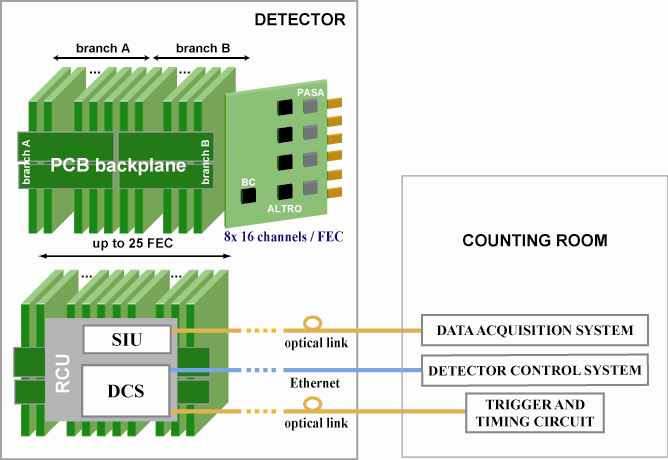
\includegraphics[width=1.0\textwidth]{images/altro.png}
     \caption{Readout schematics for the current TPC detector}
    \label{fig:altro}
\end{figure}

\section{Long Shutdown 2}
\paragraph{•}
As mentioned in \ref{sec:motivation} the \gls{lhc} ring will be shut down for about 3 years, and during that time the \gls{alice} detector will undergo a extensive upgrade.
The upgrade strategy for \gls{alice} is based on the expected increase in collision rate of 50 kHz, and will now track every collision.
Essentially this comes down to a increase by a factor of 100, compared to what is achievable today.

\paragraph{•}
To be able to handle the increase in collision rate the \gls{tpc} will receive upgrades to both its readout chambers, and front-end readout electronics.
\textit{Her skal jeg skrive mer. (Sampa, cru, etc..)}


\chapter{Problem description}
\textit{SystemC, Starting design of the simulation, plans for implementation and test runs}

\section{Simulation}
\textit{General simulation theory (Should this be in a previous chapter?)}

\subsection{Theory}
\paragraph{•}
A simulation can be seen as the imitation of a real-world system and its operations over time.
This requires a model representation of the system which is accurate enough to conduct experiments on, which produce real-like results.
The model should include key characteristics, specifications and functions of the selected system, but in a simplified fashion.
A simulation model can take many forms as it can be used in different contexts ranging from physical object such as electrical circuits, bridges, and even entire cities too abstract systems like a mathematical equation or a scientific experiment. %Source

\paragraph{•} 
As the model represent the system itself, the simulation represents its operations over a set period of time.
The simulation is normally conducted in a controlled environment that makes it possible to observe, monitor and log results.
To achieve efficient experimenting using a simulation, it should be easy to change its parameters with respect to what is being tested.

\paragraph{•}
There are many benefits of simulating a system instead of creating and test the real thing.
A simulation will in most cases be very time efficient, you can conduct the same kinds of experiments on the system in a much shorter time compared to the real thing.
This means that more information about the systems behaviour and limitations in less time, which in turn can result in a better final product.
Creating the real-world system can often be very expensive, which may limit the amount of prototypes or testproducts that are possible to create.
Therefore using results of a simulation to fine tune the specifications before starting to produce prototypes will cut unnecessary development costs by a significant margin.

\paragraph{•}
Taking the upgrade of the readout electronics for the \gls{alice} detector as an example to further address this point one can see the usefulness of not having to create multiple custom hardware components, all with different purposed specification.
In regards to the readout electronics, another important point is that the proposed designs might work well from the start, but there is always room for improvement. 
Finding out that the design doesn't need as much memory, or less optic fibre cables can impact the overall production costs.
One way to efficiently and accurately simulate hardware components is by creating a virtual computer simulation.

\subsection{Computer Simulation}
\paragraph{•}
Using computers to do simulations is in this day and age become more and more useful because of their incredible computational power, and ability to produce fast results.
%MORE stuff
\paragraph{•}
Computer simulations often becomes quite complex, and it is often wise to use existing tools to help make the process easier.
There is an array of different tools that can be used to various kinds of simulations.
They vary from complete frameworks, with user interfaces too tools which helps developers write there own simulation program.


\section{SystemC}
\textit{Explain how SystemC works, what benefits and downsides}

\section{Model Designs}
\textit{Different design patterns, and plans for the electronic}

\subsection{Zero suppression}
\subsection{Huffman Encoding}

\chapter{Solution implementation}
\textit{Code snippets, Incremental implementation stages and the final implementation, (before and after huffman), using real data vs random. Implementing fluxiation into the simulation}

\chapter{Evaluation and results}
\textit{Running the tests, results from different tests, Evaluating the final product}

\chapter{Conclusion and Future work}
\textit{Conclude the thesis, talk about the impact it has and its usefulness in future planing of the front end electronics.}

\bibliography{biblio}{}
\bibliographystyle{unsrt}
\end{document}
